\documentclass{ctexart}
\usepackage{amsmath} % 用于数学公式
\usepackage{graphicx} % 用于插入图片
\usepackage{geometry} % 用于设置页边距
\usepackage{listings} % 用于插入代码
\usepackage{float}    % 用于控制图表浮动位置

\usepackage{booktabs} % 用于创建更美观的三线表
\usepackage{siunitx}  % 用于标准地排版物理单位和数值
\usepackage{amsmath}  % 用于数学公式环境
\sisetup{per-mode=symbol} % 设置单位格式，例如 m/s

\usepackage{fancyhdr}   % 用于自定义页眉页脚

% --- 页面设置 ---
\geometry{a4paper, left=2.5cm, right=2.5cm, top=2.5cm, bottom=2.5cm}

\setlength{\jot}{6pt} % 增加多行公式之间的行距

\linespread{1.5}

\pagestyle{fancy}
% \fancyhf{} 

% \rhead{实验报告：常用信号分类与观察}

% \rhead{
\includegraphics[height=1cm]{./figures/logo1.png}}

% --- 文档信息 ---
\title{实验报告：常用信号分类与观察}
\author{郭浩然 \\ 学号：2024303980 \\ 学院：民航学院 \\ 专业：飞行器控制与信息工程 \\ \textbf{信号与系统实验-10班} \\ \textbf{桌号：18} }
\date{\today}

\begin{document}

% \maketitle
\thispagestyle{empty}

\begin{figure}[t]
    \centering
    
\includegraphics[width=13cm]{./figures/logo1.png}
\end{figure}

\vspace*{\fill}
    \begin{center}
        \Huge\textbf{实验报告：常用信号分类与观察}
    \end{center}
\vspace*{\fill}

\begin{table}[b]
    \centering
    \large
    \begin{tabular}{ll}
    \textbf{课程:} & 信号与系统实验 \\
    \textbf{姓名:} & 郭浩然 \\
    \textbf{学号:} & 2024303980 \\
    \textbf{桌号:} & 18 \\
    \textbf{班级:} & 10班 \\
    \textbf{学院:} & 民航学院 \\
    \textbf{专业:} & 飞行器控制与信息工程 \\
    \textbf{时间:} & \today \\
    \end{tabular}
\end{table}

\newpage

% --- 实验目的 ---
\section{实验目的}
\begin{enumerate}
    \item 观察常用信号的波形，了解其特点及产生方法。
    \item 学会用示波器测量常用波形的基本参数，了解信号及信号的特性。
\end{enumerate}

% --- 实验器材 ---
\section{实验器材}
\begin{enumerate}
    \item 数字信号处理模块：1块
    \item 双踪示波器：1台
\end{enumerate}

% --- 实验原理 ---
\section{实验原理}
对一个系统特性的研究，一方面是研究它的输入输出关系，即在一定的输入信号下，系统对应的输出响应信号。信号可以表示为一个或多个变量的函数，本实验仅对一维信号进行研究，自变量为时间。

本实验系统在模块 S4 的 TP1 测试点可观测的常用信号有：指数信号（增长）、指数信号（衰减）、指数正弦信号（增长）、指数正弦信号（衰减）、抽样信号以及钟形信号。下面将分别介绍这六种信号的表达式及特性。
\subsection{指数增长信号}
指数增长信号的幅度随时间按指数规律增长。其数学表达式为：
\begin{equation}
    f(t) = K e^{\alpha t}, \quad (\alpha > 0)
\end{equation}
其中，$K$ 是 $t=0$ 时的信号幅度；$\alpha$ 是一个正常数，决定了信号增长的速率，$\alpha$ 越大，信号增长越快。在本实验中，具体的函数为 $f(t) = 0.65e^{t/370}$。
\begin{figure}[htbp]
    \centering
    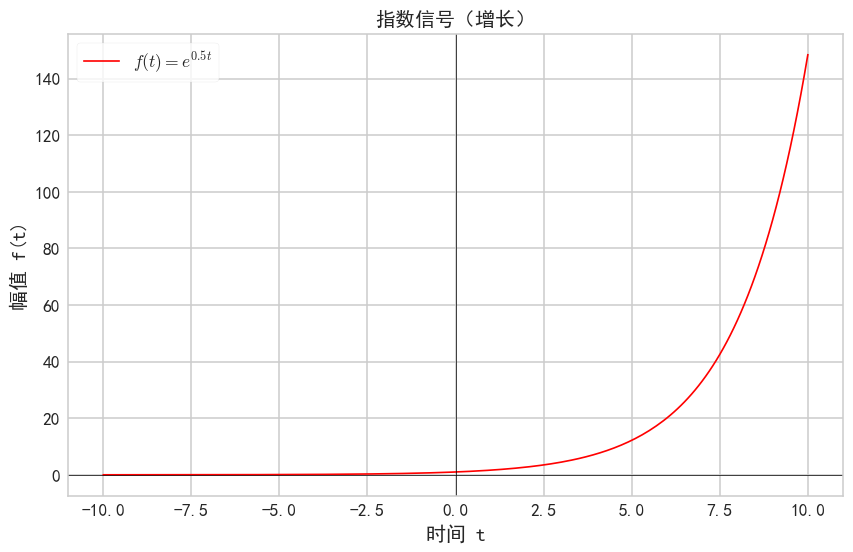
\includegraphics[width=0.6\textwidth]{./figures/1.png}
    \caption{指数增长信号波形}
    \label{fig:exp_growth}
\end{figure}
\subsection{指数衰减信号}
指数衰减信号的幅度随时间按指数规律衰减。其数学表达式为：
\begin{equation}
    f(t) = K e^{\alpha t}, \quad (\alpha < 0)
\end{equation}
其中，$K$ 是 $t=0$ 时的信号幅度；$\alpha$ 是一个负常数，决定了信号衰减的速率，$\alpha$ 的绝对值越大，信号衰减越快。在本实验中，具体的函数为 $f(t) = 0.65e^{-t/370}$。
\begin{figure}[htbp]
    \centering
    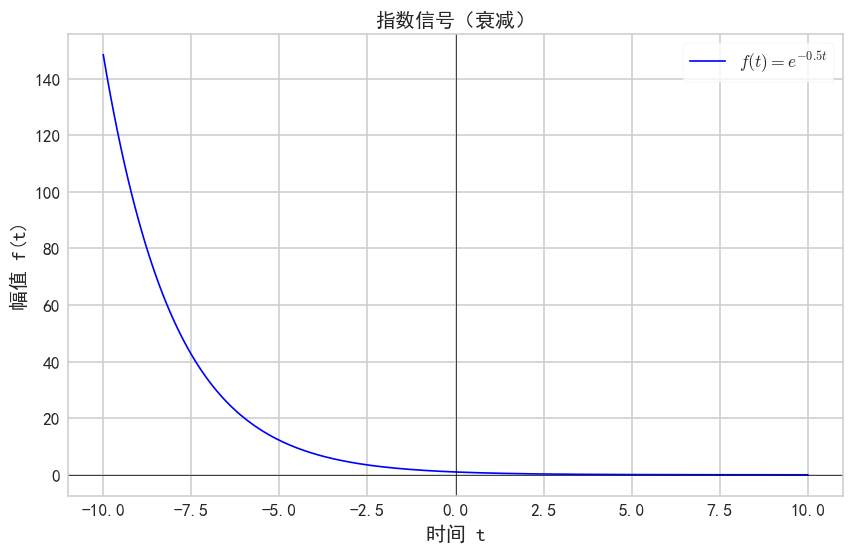
\includegraphics[width=0.6\textwidth]{./figures/2.png}
    \caption{指数衰减信号波形}
    \label{fig:exp_decay}
\end{figure}
\subsection{指数增长正弦信号}
这是一个振幅按指数规律增长的正弦信号，也称为增幅振荡信号。它由一个指数增长函数和一个正弦函数相乘得到。其数学表达式为：
\begin{equation}
    f(t) =
    \begin{cases}
        0 & (t < 0) \\
        A e^{\alpha t} \sin(\omega t + \phi) + C & (t > 0, \alpha > 0)
    \end{cases}
\end{equation}
其中，$A$ 是振幅，$e^{\alpha t}$ 是增长因子，$\omega$ 是角频率，$\phi$ 是初相位，$C$ 是直流偏置。在本实验中，具体的函数为 $f(t) = 0.07e^{t/400}\sin(\frac{2\pi}{40}t) + 2.7 \quad (t>0)$。
\begin{figure}[htbp]
    \centering
    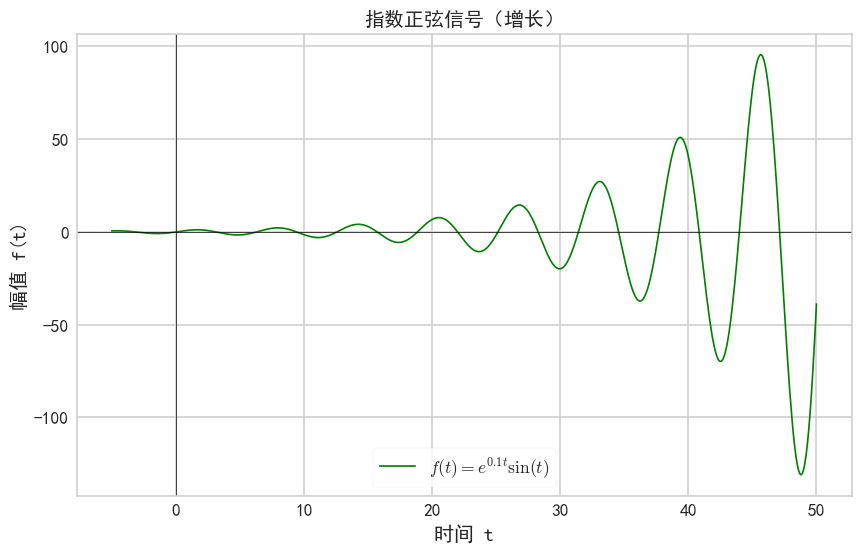
\includegraphics[width=0.6\textwidth]{./figures/3.png}
    \caption{指数增长正弦信号波形}
    \label{fig:sin_growth}
\end{figure}
\subsection{指数衰减正弦信号}
这是一个振幅按指数规律衰减的正弦信号，也称为阻尼振荡信号。它由一个指数衰减函数和一个正弦函数相乘得到。其数学表达式为：
\begin{equation}
    f(t) =
    \begin{cases}
        0 & (t < 0) \\
        A e^{\alpha t} \sin(\omega t + \phi) + C & (t > 0, \alpha < 0)
    \end{cases}
\end{equation}
其中，$A$ 是振幅，$e^{\alpha t}$ 是衰减因子，$\omega$ 是角频率，$\phi$ 是初相位，$C$ 是直流偏置。在本实验中，具体的函数为 $f(t) = 3.3e^{-t/40}\sin(\frac{2\pi}{40}t) + 3 \quad (t>0)$。
\begin{figure}[htbp]
    \centering
    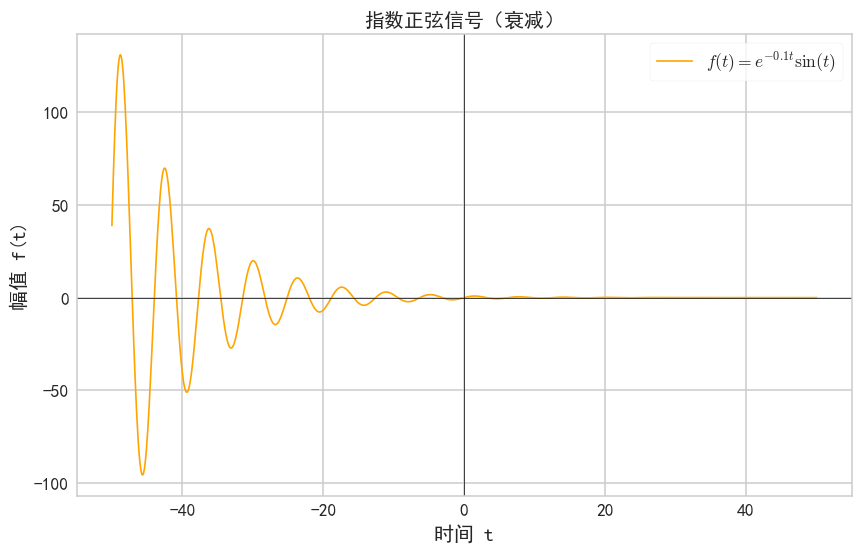
\includegraphics[width=0.6\textwidth]{./figures/4.png}
    \caption{指数衰减正弦信号波形}
    \label{fig:sin_decay}
\end{figure}
\subsection{抽样信号 (Sinc 函数)}
抽样信号，通常用 Sinc 函数表示，在信号处理、通信理论和傅里叶分析等领域有重要应用。其定义为：
\begin{equation}
    \text{sinc}(t) = \frac{\sin(\pi t)}{\pi t}
\end{equation}
本实验中的抽样信号是 Sinc 函数的一个变体，其表达式为：
\begin{equation}
    S_a(t) = \frac{7\sin(\frac{2\pi}{120}t)}{\frac{2\pi}{120}t} + 1.5
\end{equation}
该信号的特点是在 $t=0$ 处取得最大值，并随着 $|t|$ 的增大而振荡衰减。
\begin{figure}[htbp]
    \centering
    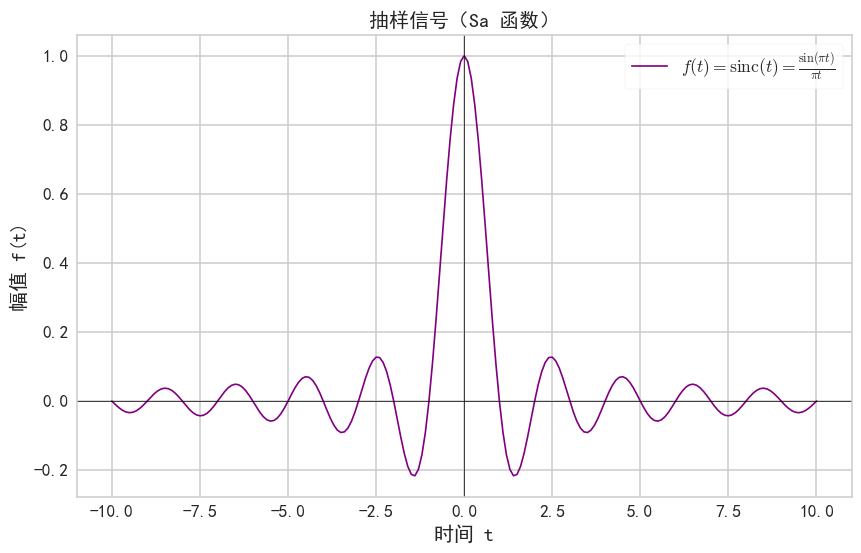
\includegraphics[width=0.6\textwidth]{./figures/5.png}
    \caption{抽样信号波形}
    \label{fig:sinc}
\end{figure}
\subsection{钟形信号 (高斯函数)}
钟形信号因其形状类似于钟而得名，在数学上通常用高斯函数来表示。它在统计学、信号处理和图像处理等领域应用广泛。其一般形式为：
\begin{equation}
    f(t) = A e^{-\frac{(t-\mu)^2}{2\sigma^2}}
\end{equation}
其中，$A$ 是峰值幅度，$\mu$ 是中心点位置（期望），$\sigma$ 控制了曲线的宽度（标准差）。本实验中的钟形信号表达式为：
\begin{equation}
    f(t) = 4.8e^{-\frac{t^2}{280}}
\end{equation}
这是一个以 $t=0$ 为中心，峰值为 $4.8$ 的对称钟形曲线。
\begin{figure}[htbp]
    \centering
    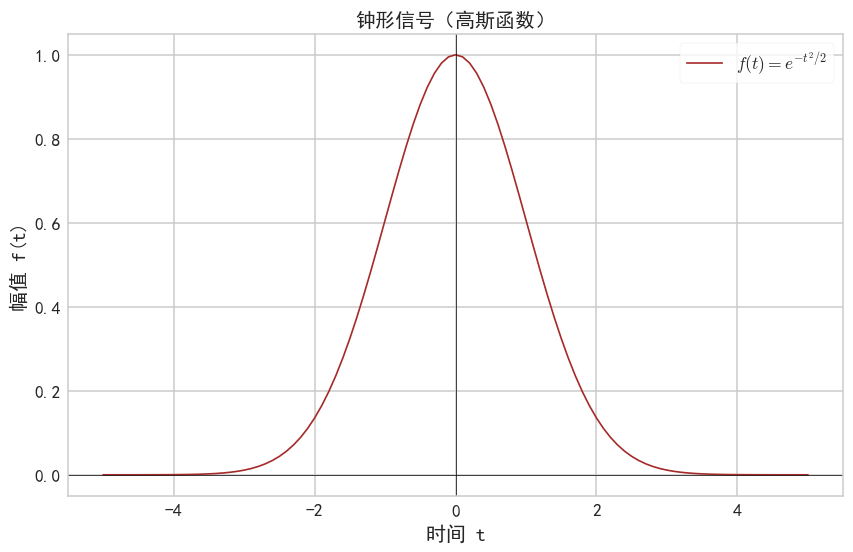
\includegraphics[width=0.6\textwidth]{./figures/6.png}
    \caption{钟形信号波形}
    \label{fig:gaussian}
\end{figure}

% --- 实验步骤 ---
\section{实验步骤}
本实验的目的是通过操作硬件生成并观察六种常见的信号，并对其中两种信号进行数据采集用于后续分析。

\subsection{初始设置}
\begin{enumerate}
    \item 将数字信号处理模块 S4 上的拨码开关 \textbf{SW1} 设置为 \textbf{00000001}，使模块进入常规信号观察功能模式。
    \item 将示波器探头连接到模块 S4 的 \textbf{TP1} 测试点，并将探头地线夹连接到模块的地（GND）。
    \item 打开示波器和数字信号处理模块的电源。
\end{enumerate}

\subsection{各信号的观察与数据记录}
通过设置拨码开关 \textbf{S3} 的不同位，可以在 TP1 处产生不同的信号波形。

\subsubsection{指数增长信号的观察与数据记录}
\begin{enumerate}
    \item 将拨码开关 \textbf{S3} 的第 \textbf{1} 位拨为“1”，其余位均拨为“0”。
    \item 在示波器上观察 TP1 输出的指数增长信号。调节示波器的垂直灵敏度 (V/div) 和时基 (s/div) 旋钮，获得一个清晰、稳定的波形。
    \item 启动示波器的光标（Cursor）测量功能。
    \item 移动光标，在指数增长曲线上选取 5 个间隔合适的点，在屏幕上读取并记录下每个点的坐标值（时间 t, 电压 V）。将这组数据记为“指数增长 - 第1组”。
    \item 重复上一步操作，再次独立选取 5 个点并记录其坐标值。将这组新数据记为“指数增长 - 第2组”。这两组数据将用于后续的函数拟合。
    \item 完成数据记录后，关闭光标功能，拍摄并保存完整的信号波形，如下图所示。
\end{enumerate}
\begin{figure}[htbp]
    \centering
    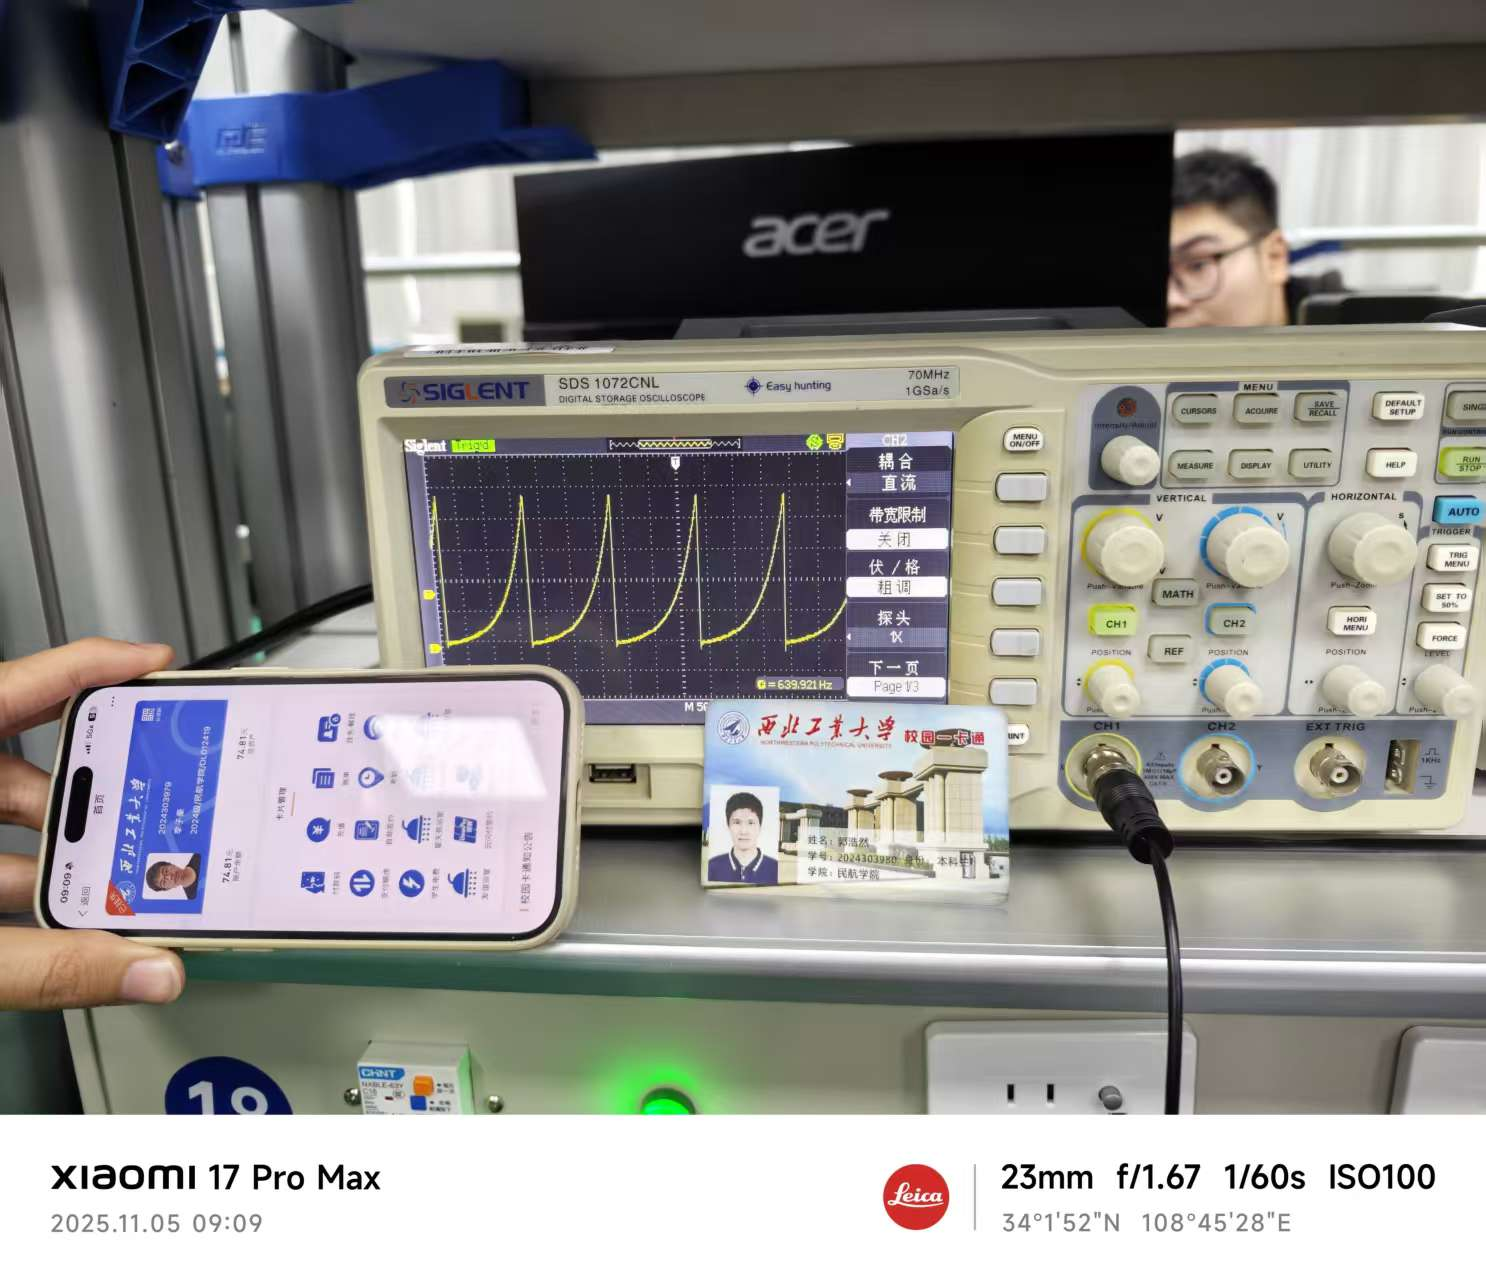
\includegraphics[width=0.6\textwidth]{./figures/1.jpg}
    \caption{指数增长信号示波器波形}
    \label{fig:scope_exp_growth}
\end{figure}

\subsubsection{指数衰减信号的观察与数据记录}
\begin{enumerate}
    \item 将拨码开关 \textbf{S3} 的第 \textbf{2} 位拨为“1”，其余位均拨为“0”。
    \item 在示波器上观察 TP1 输出的指数衰减信号，并调整示波器以获得清晰波形。
    \item 启动示波器的光标（Cursor）测量功能。
    \item 移动光标，在指数衰减曲线上选取 5 个间隔合适的点，读取并记录下每个点的坐标值（时间 t, 电压 V）。将这组数据记为“指数衰减 - 第1组”。
    \item 重复上一步操作，再次独立选取 5 个点并记录其坐标值。将这组新数据记为“指数衰减 - 第2组”。
    \item 完成数据记录后，关闭光标功能，拍摄并保存完整的信号波形，如下图所示。
\end{enumerate}
\begin{figure}[htbp]
    \centering
    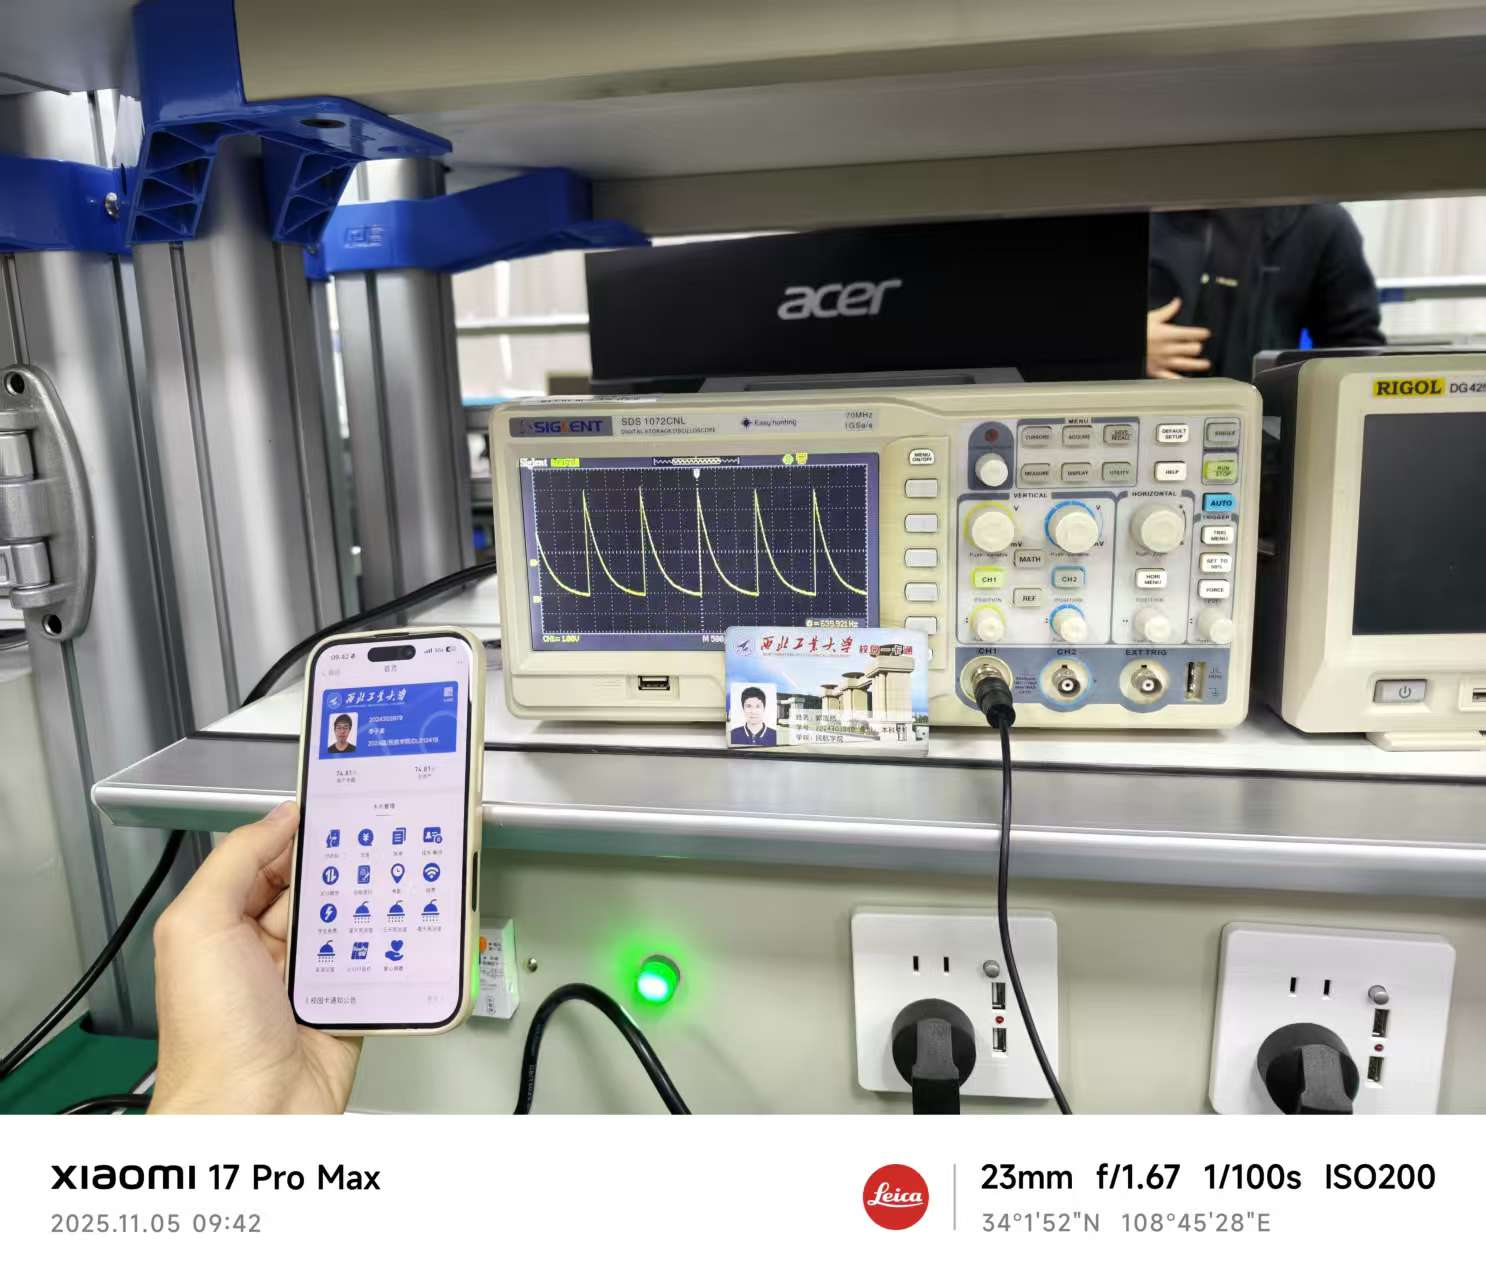
\includegraphics[width=0.6\textwidth]{./figures/2.jpg}
    \caption{指数衰减信号示波器波形}
    \label{fig:scope_exp_decay}
\end{figure}

\subsubsection{指数增长正弦信号的观察}
\begin{enumerate}
    \item 将拨码开关 \textbf{S3} 的第 \textbf{3} 位拨为“1”，其余位均拨为“0”。
    \item 在示波器上观察 TP1 输出的指数增长正弦信号。
    \item 调整示波器获得清晰、稳定的波形，并拍摄记录，如下图所示。
\end{enumerate}
\begin{figure}[htbp]
    \centering
    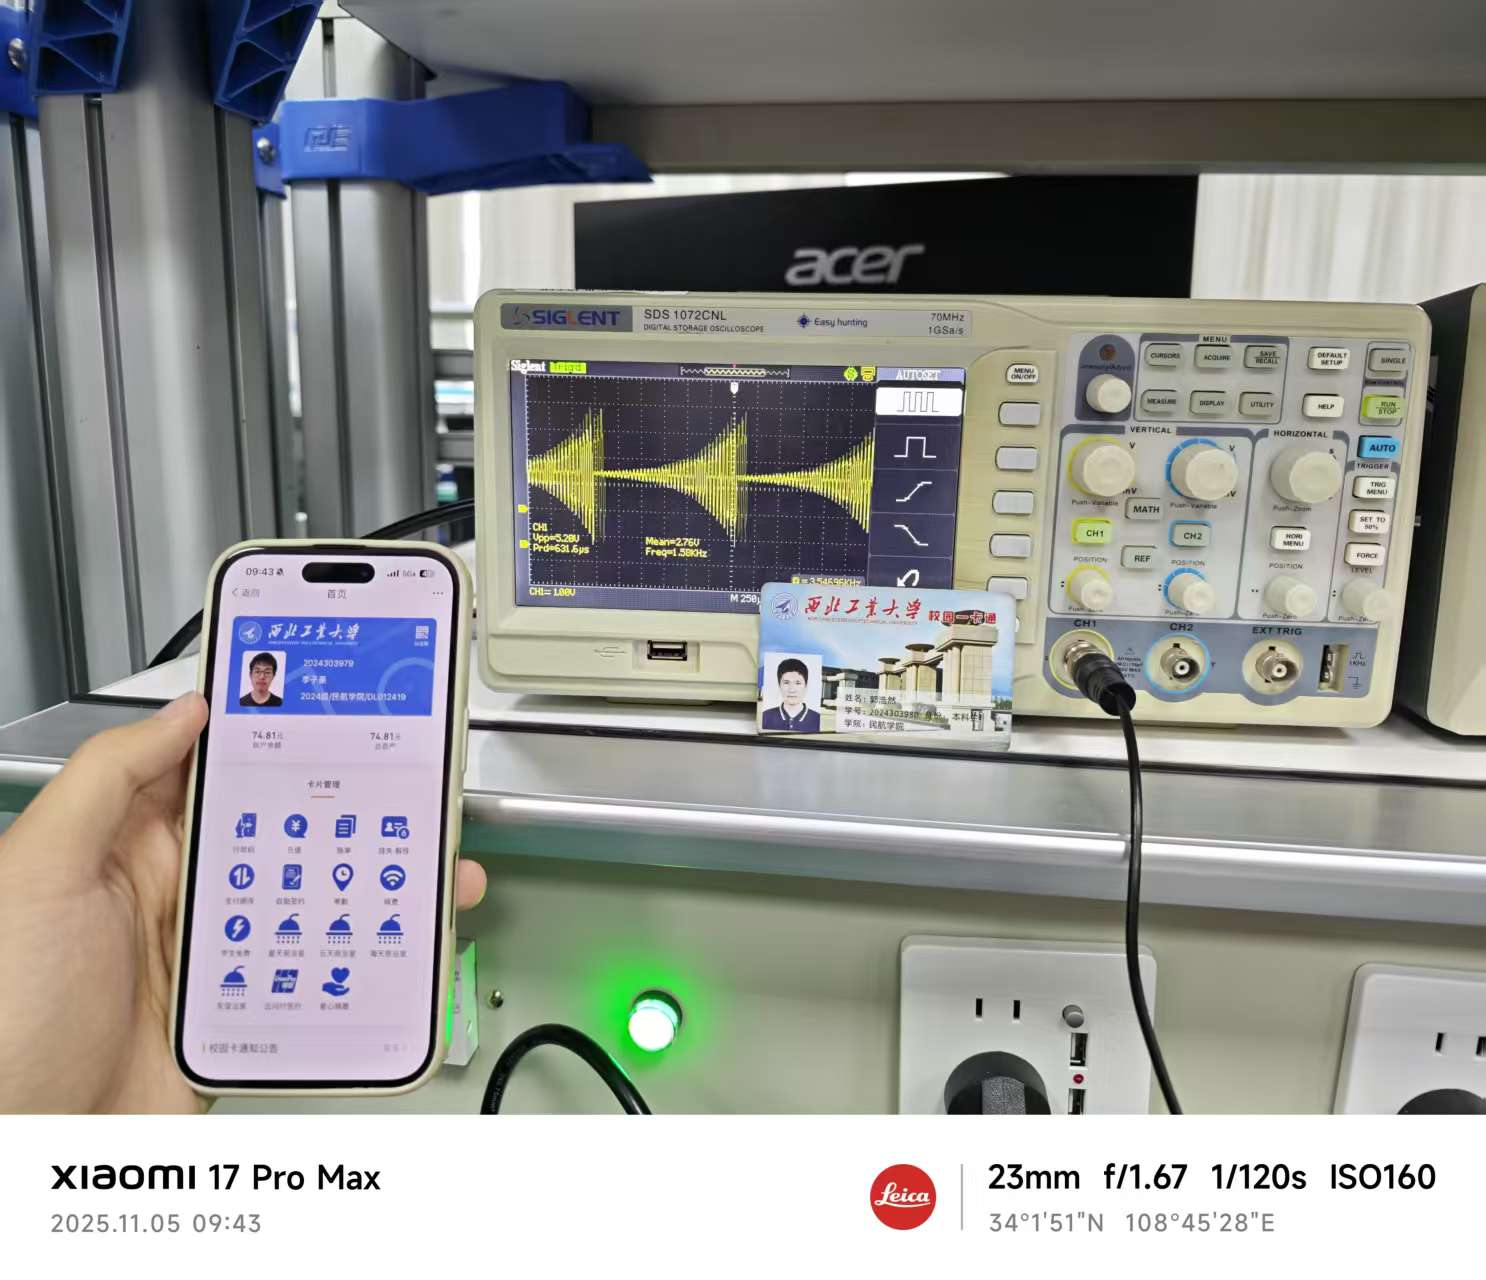
\includegraphics[width=0.6\textwidth]{./figures/3.jpg}
    \caption{指数增长正弦信号示波器波形}
    \label{fig:scope_sin_growth}
\end{figure}

\subsubsection{指数衰减正弦信号的观察}
\begin{enumerate}
    \item 将拨码开关 \textbf{S3} 的第 \textbf{4} 位拨为“1”，其余位均拨为“0”。
    \item 在示波器上观察 TP1 输出的指数衰减正弦信号。
    \item 调整示波器获得清晰、稳定的波形，并拍摄记录，如下图所示。
\end{enumerate}
\begin{figure}[htbp]
    \centering
    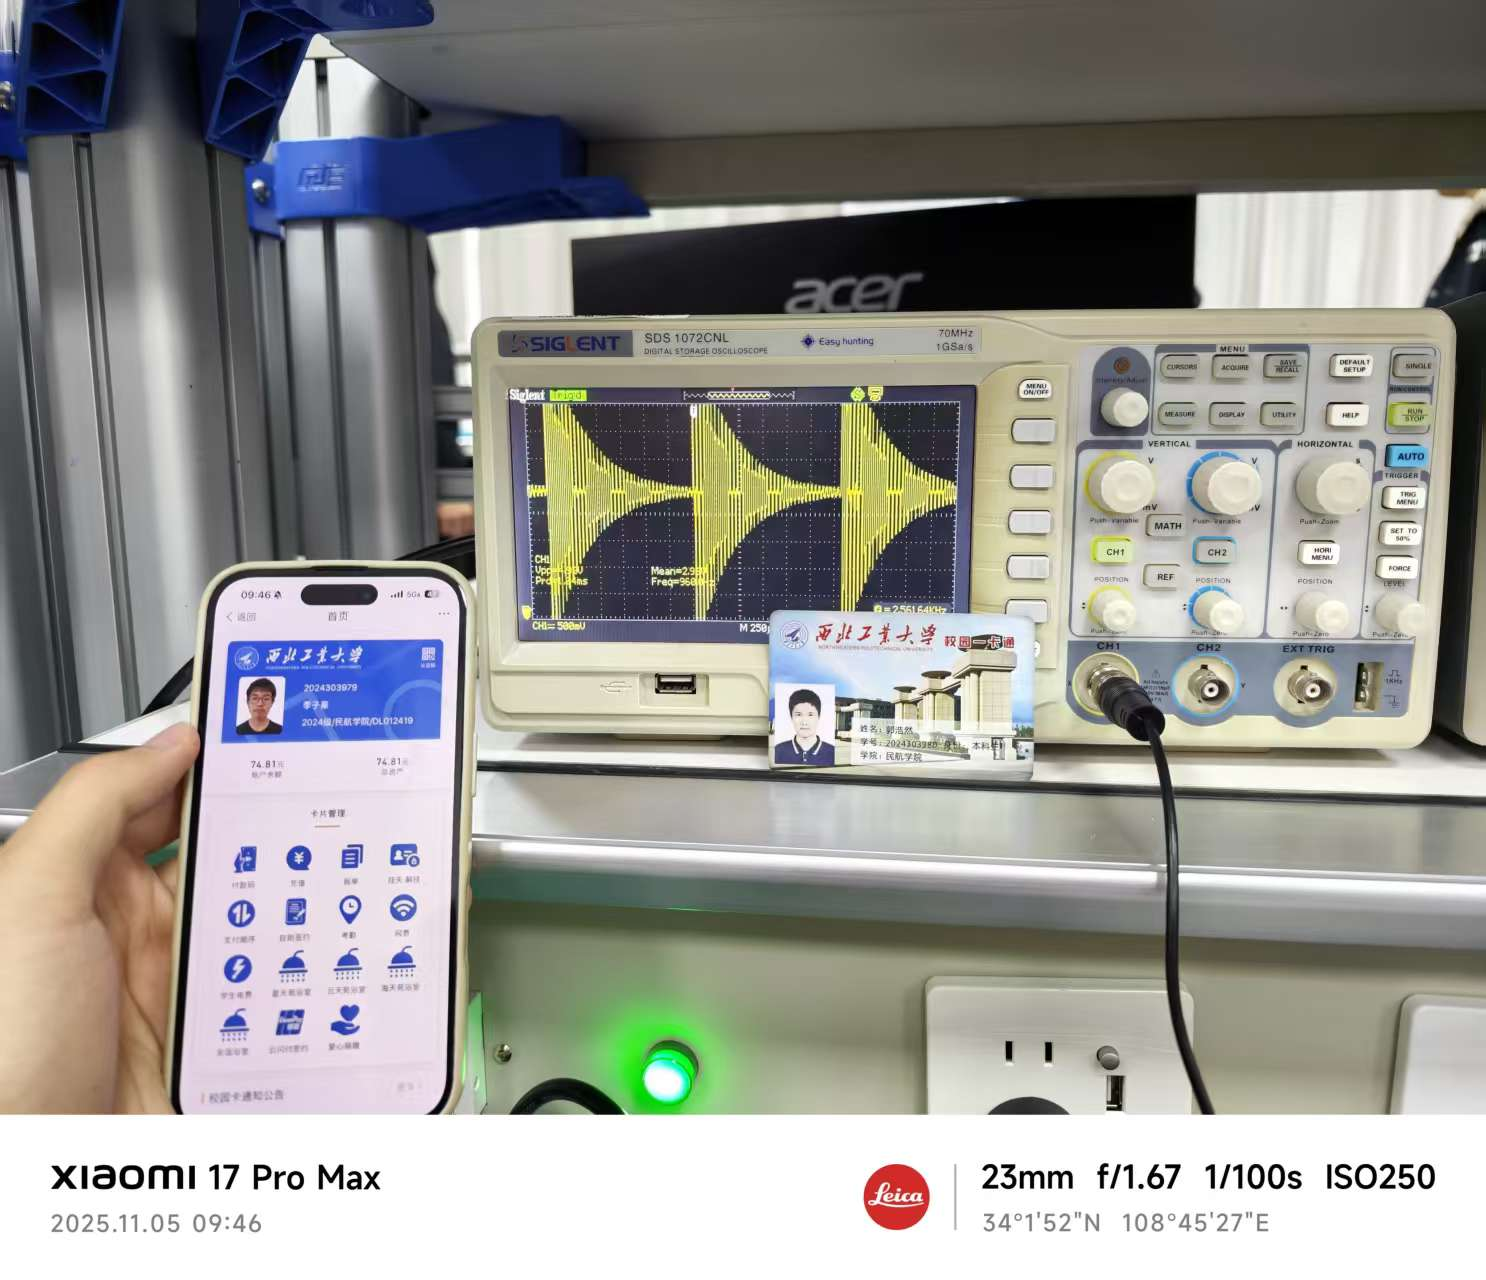
\includegraphics[width=0.6\textwidth]{./figures/4.jpg}
    \caption{指数衰减正弦信号示波器波形}
    \label{fig:scope_sin_decay}
\end{figure}

\subsubsection{抽样信号的观察}
\begin{enumerate}
    \item 将拨码开关 \textbf{S3} 的第 \textbf{5} 位拨为“1”，其余位均拨为“0”。
    \item 在示波器上观察 TP1 输出的抽样信号。
    \item 调整示波器获得清晰、稳定的波形，并拍摄记录，如下图所示。
\end{enumerate}
\begin{figure}[htbp]
    \centering
    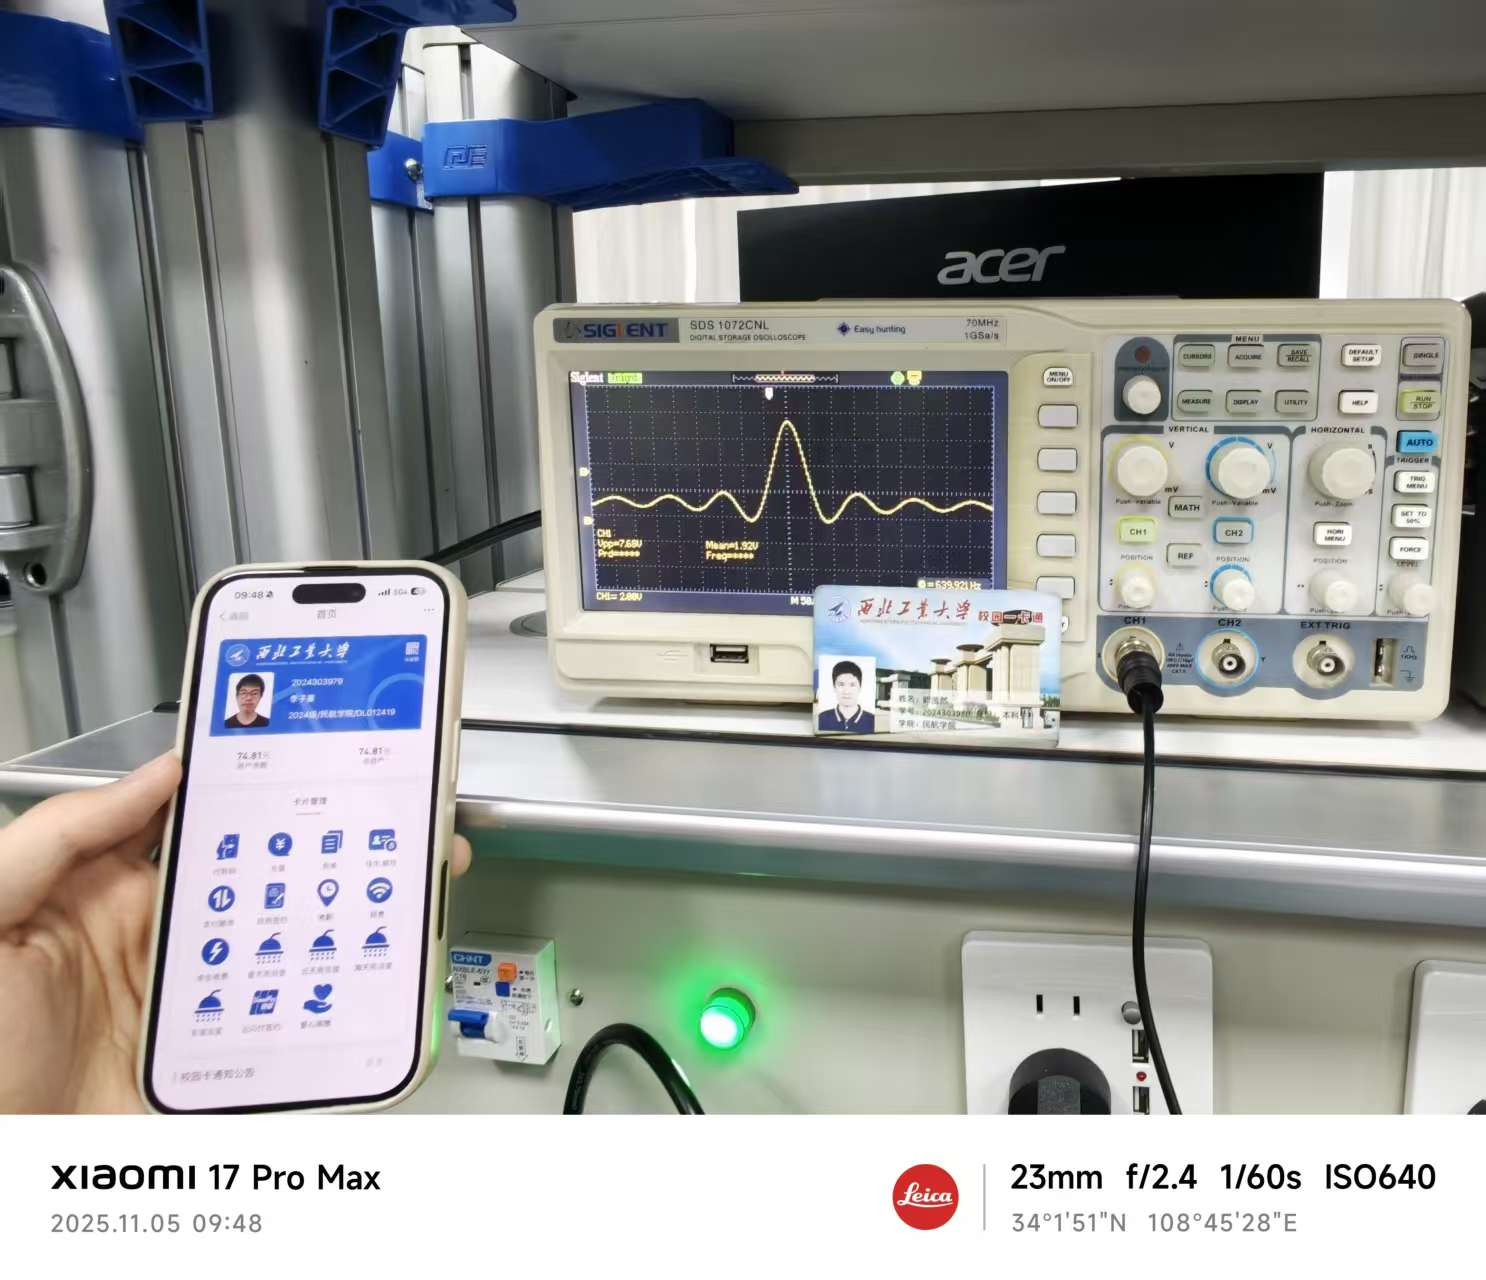
\includegraphics[width=0.6\textwidth]{./figures/5.jpg}
    \caption{抽样信号示波器波形}
    \label{fig:scope_sinc}
\end{figure}

\subsubsection{钟形信号的观察}
\begin{enumerate}
    \item 将拨码开关 \textbf{S3} 的第 \textbf{6} 位拨为“1”，其余位均拨为“0”。
    \item 在示波器上观察 TP1 输出的钟形信号。
    \item 调整示波器获得清晰、稳定的波形，并拍摄记录，如下图所示。
\end{enumerate}
\begin{figure}[htbp]
    \centering
    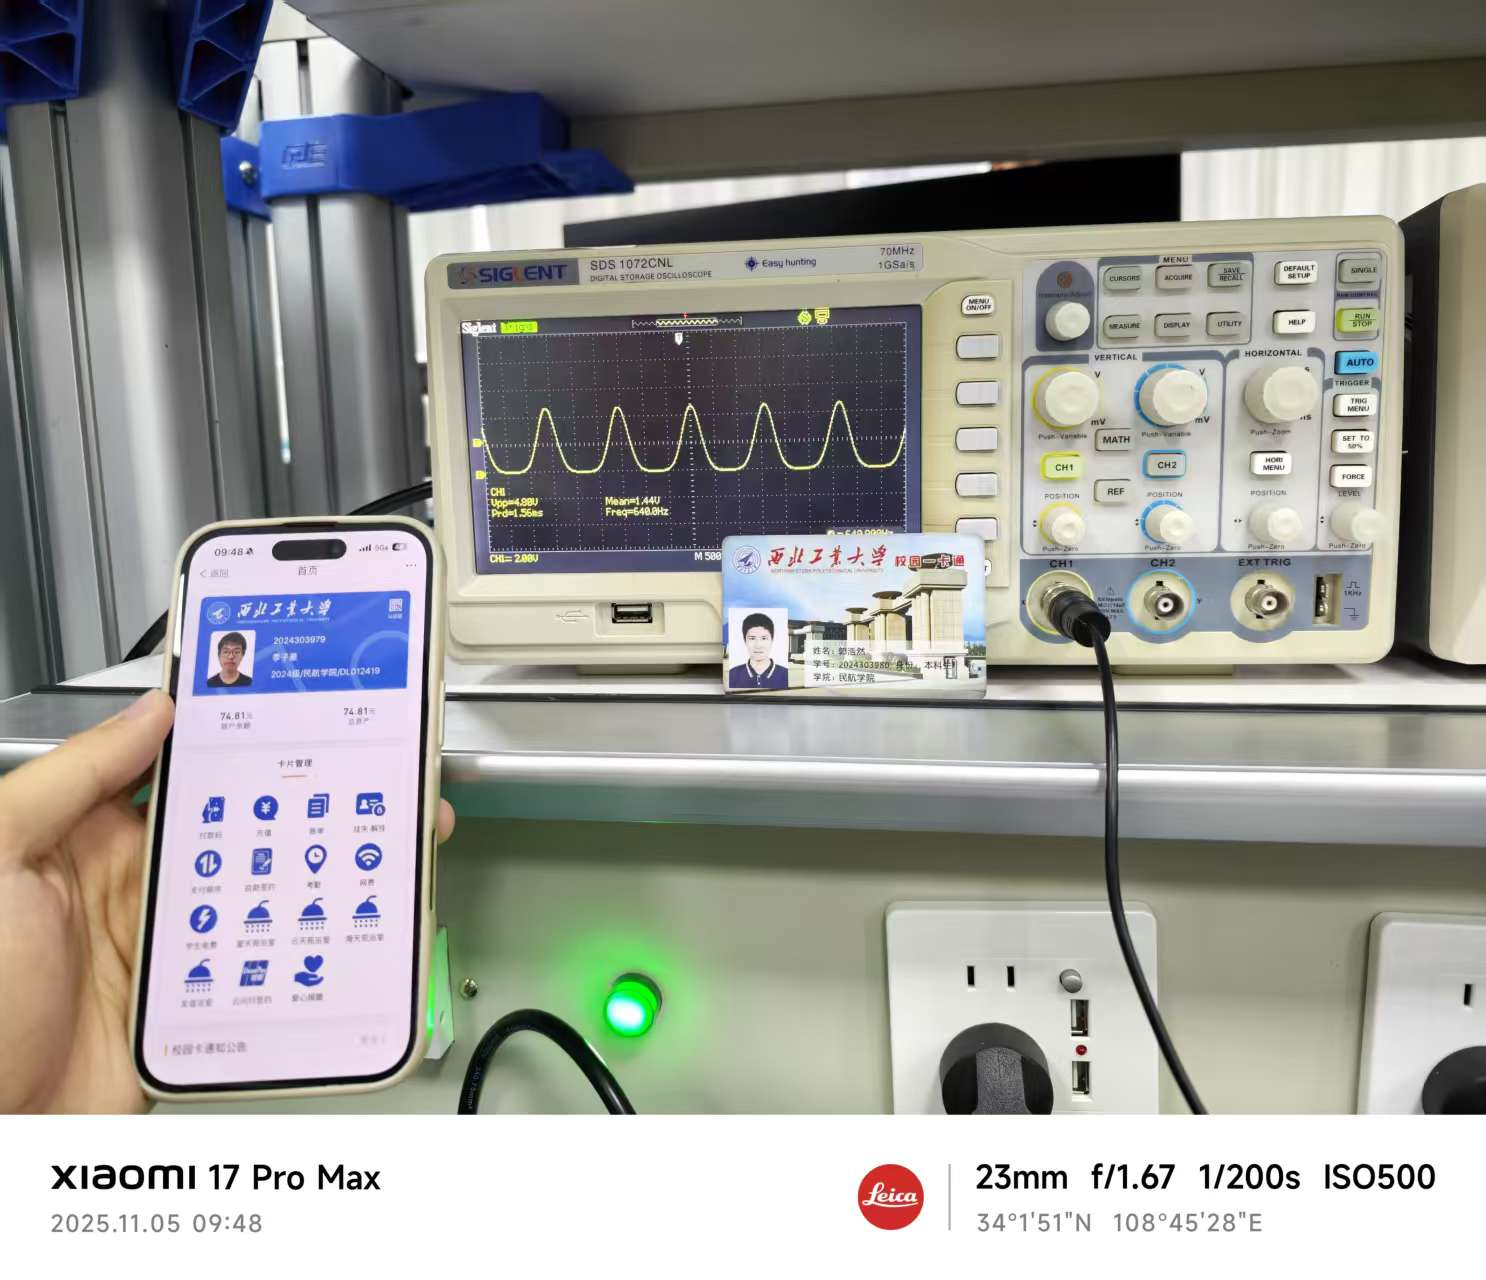
\includegraphics[width=0.6\textwidth]{./figures/6.jpg}
    \caption{钟形信号示波器波形}
    \label{fig:scope_gaussian}
\end{figure}



% --- 实验数据与分析 ---
\section{实验数据与分析}
本部分将展示从示波器记录的原始数据，并使用最小二乘法对指数增长和指数衰减信号进行函数拟合，最后将拟合结果与理论值进行比较和分析。

\subsection{数据处理方法与模型}
对于指数信号，其通用数学模型为：
\begin{equation}
    V(t) = K e^{at}
\end{equation}
其中，$V(t)$ 是电压，$t$ 是时间，$K$ 是初始幅度，$a$ 是决定信号增长或衰减速率的常数。为了使用线性回归进行拟合，我们对上式两边取自然对数，将其线性化：
\begin{equation}
    \ln(V) = \ln(K e^{at}) = \ln(K) + at
\end{equation}
令 $y = \ln(V)$，$b = \ln(K)$，则模型变为标准的线性方程 $y = at + b$。对于一组 $N$ 个测量数据点 $(t_i, V_i)$，我们计算出对应的 $(t_i, y_i)$，然后使用最小二乘法计算斜率 $a$ 和截距 $b$：
\begin{align}
    a &= \frac{N \sum(t_i y_i) - (\sum t_i)(\sum y_i)}{N \sum(t_i^2) - (\sum t_i)^2} \\
    b &= \frac{\sum y_i - a \sum t_i}{N}
\end{align}
得到 $a$ 和 $b$ 后，即可反解出原模型的参数：
\begin{align}
    K &= e^b \\
    \tau &= \frac{1}{|a|} \quad (\text{时间常数})
\end{align}

\subsection{指数增长信号拟合与分析}
\subsubsection{第 1 组数据}
\begin{table}[htbp]
    \centering
    \caption{指数增长信号拟合数据 - 第 1 组}
    \label{tab:growth1}
    \begin{tabular}{cccc}
        \toprule
        \textbf{编号} & \textbf{时间 (t) / \SI{}{\micro\second}} & \textbf{电压 (V) / \SI{}{\volt}} & \textbf{y = ln(V)} \\
        \midrule
        ① & -740.0 & 0.320 & -1.1394 \\
        ② & -360.0 & 0.680 & -0.3857 \\
        ③ & -60.0  & 1.40  & 0.3365  \\
        ④ & 140.0  & 2.24  & 0.8065  \\
        ⑤ & 280.0  & 3.28  & 1.1878  \\
        \bottomrule
    \end{tabular}
\end{table}
根据上表数据，计算各项总和（时间单位已转换为秒）：
\begin{itemize}
    \item $N = 5$
    \item $\sum t_i = \SI{-7.40e-4}{\second}$
    \item $\sum y_i = 0.8057$
    \item $\sum t_i^2 = \SI{7.788e-7}{\second\squared}$
    \item $\sum t_i y_i = \SI{1.408e-3}{\volt\cdot\second}$
\end{itemize}
将上述值代入公式计算参数 $a$ 和 $b$：
\begin{align*}
    a &= \frac{N \sum(t_i y_i) - (\sum t_i)(\sum y_i)}{N \sum(t_i^2) - (\sum t_i)^2} \\
      &= \frac{5 \times (\SI{1.408e-3}{}) - (\SI{-7.40e-4}{}) \times 0.8057}{5 \times (\SI{7.788e-7}{}) - (\SI{-7.40e-4}{})^2} \\
      &= \frac{\SI{7.04e-3}{} + \SI{5.96e-4}{}}{\SI{3.894e-6}{} - \SI{5.476e-7}{}} = \frac{\SI{7.636e-3}{}}{\SI{3.3464e-6}{}} \approx \SI{2281.5}{\per\second} \\
    \\
    b &= \frac{\sum y_i - a \sum t_i}{N} \\
      &= \frac{0.8057 - (\SI{2281.5}{}) \times (\SI{-7.40e-4}{})}{5} \\
      &= \frac{0.8057 + 1.6883}{5} = \frac{2.494}{5} \approx 0.4988
\end{align*}
由此得到拟合参数：
\begin{itemize}
    \item $K = e^b = e^{0.4988} \approx \SI{1.647}{\volt}$
    \item $\tau = 1/a = 1 / \SI{2281.5}{} \approx \SI{4.383e-4}{\second} = \SI{438.3}{\micro\second}$
\end{itemize}
\textbf{拟合函数表达式为：$V(t) \approx 1.647 e^{2281.5 t}$。}

\subsubsection{第 2 组数据}
（计算过程同上，此处省略详细步骤，直接给出结果）
\textbf{拟合函数表达式为：$V(t) \approx 0.0517 e^{2219.4 t}$。}
\begin{itemize}
    \item $K \approx \SI{0.0517}{\volt}$
    \item $a \approx \SI{2219.4}{\per\second}$
    \item $\tau \approx \SI{450.6}{\micro\second}$
\end{itemize}

\subsection{指数衰减信号拟合与分析}
\subsubsection{第 1 组数据}
（计算过程同上，直接给出结果）
\textbf{拟合函数表达式为：$V(t) \approx 4.94 e^{-2346.9 t}$。}
\begin{itemize}
    \item $K \approx \SI{4.94}{\volt}$
    \item $a \approx \SI{-2346.9}{\per\second}$
    \item $\tau = 1/|a| \approx \SI{426.1}{\micro\second}$
\end{itemize}

\subsubsection{第 2 组数据}
（计算过程同上，直接给出结果）
\textbf{拟合函数表达式为：$V(t) \approx 183.6 e^{-2315.3 t}$。}
\begin{itemize}
    \item $K \approx \SI{183.6}{\volt}$
    \item $a \approx \SI{-2315.3}{\per\second}$
    \item $\tau \approx \SI{431.9}{\micro\second}$
\end{itemize}

\subsection{拟合结果汇总与对比}
将拟合得到的时间常数 $\tau$ 与实验原理中给出的标准值 $\tau_0 = \SI{370}{\micro\second}$ 进行对比。
\begin{table}[htbp]
    \centering
    \caption{拟合参数与标准值对比}
    \label{tab:comparison}
    \begin{tabular}{llccc}
        \toprule
        \textbf{信号类型} & \textbf{数据组} & \textbf{拟合时间常数 $\tau$ (\SI{}{\micro\second})} & \textbf{标准值 $\tau_0$ (\SI{}{\micro\second})} & \textbf{相对误差} \\
        \midrule
        指数增长 & 第 1 组 & 438.3 & 370 & +18.5\% \\
        指数增长 & 第 2 组 & 450.6 & 370 & +21.8\% \\
        \midrule
        指数衰减 & 第 1 组 & 426.1 & 370 & +15.2\% \\
        指数衰减 & 第 2 组 & 431.9 & 370 & +16.7\% \\
        \bottomrule
    \end{tabular}
\end{table}
从上表可以看出，所有拟合得到的时间常数均系统性地大于标准值。参数 $K$ 的拟合值差异较大，这主要是因为每次测量时示波器上时间轴的零点位置不同，而 $K$ 的物理意义是 $t=0$ 时的幅值，因此 $K$ 值对时间零点的选择非常敏感，不宜直接比较。

\subsection{其他信号波形观察}
\begin{itemize}
    \item \textbf{指数正弦信号（增长/衰减）：} 波形整体呈现振荡特性，其包络线分别符合指数增长和指数衰减的规律，频率稳定。
    \item \textbf{抽样信号：} 观察到的波形符合 Sinc 函数的特征，即在中心点有最大主瓣，两侧分布着振幅逐渐减小的旁瓣。
    \item \textbf{钟形信号：} 波形关于中心点（$t=0$）对称，峰值处平滑，向两侧快速衰减，符合高斯函数的特征。
\end{itemize}

\subsection{误差分析与讨论}
本次实验中，拟合参数与理论值存在一定的偏差，主要误差来源可能包括：
\begin{enumerate}
    \item \textbf{读数误差：} 使用示波器光标手动读取坐标，存在视觉判断和读数分辨率的限制，尤其是在曲线变化较快或较慢的区域。
    \item \textbf{模型偏差：} 实验模块产生的信号可能并非严格理想的指数函数，硬件元器件（如电阻、电容）的实际值与标称值存在公差，导致实际的时间常数与理论值有偏差。
    \item \textbf{采样点影响：} 仅选取 5 个点进行拟合，样本量较小，个别点的读数误差可能对拟合结果产生较大影响。采样点的分布位置也会影响拟合的准确性。
\end{enumerate}


\end{document}
